\chapter{Podstawy teoretyczne}

Problem kategoryzacji obrazów wpisuje się w dziedzinę rozpoznawania obrazów. Zadanie to polega na rozpoznaniu przynależności różnych rodzajów obiektów do pewnych klas\cite{Tad91} i jest częścią większego zagadnienia, które określa się jako uczenie maszynowe.

\section{Uczenie maszynowe}

Uczenie maszynowe jest zagadnieniem interdyscyplinarnym z pogranicza informatyki, statystyki i sztucznej inteligencji, które zajmuje się tworzeniem systemów mogących doskonalić się za pomocą dostarczanych danych.

Systemy te ulegają nieustannej modyfikacji, zmieniają swoje wewnętrzne parametry po to by osiągnąć korzyści takie jak zwiększenie efektywności lub wydajności działania. Ważną cechą jest to, że jakkolwiek zmiany te zachodzą na podstawie czynników zewnętrznych to jednak dokonują się w systemie autonomicznie. System, który się uczy zmienia sam siebie na lepsze\cite{CICHOSZ00}.

\section{Uczenie nadzorowane i nienadzorowane}

W uczeniu maszynowym możemy wyróżnić dwa zasadnicze podejścia: uczenie nadzorowane i nienadzorowane. Różnica pomiędzy nimi polega na obecności w uczeniu nadzorowanym tzw. nauczyciela, który stanowi źródło informacji trenującej. Posługując się analogiczną terminologią, system który podlega nauce określa się jako ucznia. Na rys. \ref{fig:supervised-learning} przedstawiono schemat uczenia maszynowego z użyciem nauczyciela.

\begin{figure}[h]
	\centering
	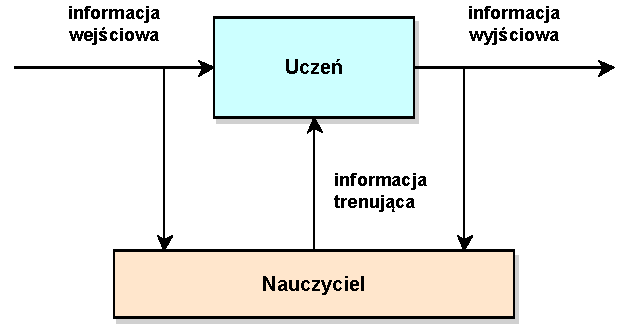
\includegraphics{graphics/01_podstawy_teoretyczne/supervised-learning.pdf}
	\caption{Uczenie maszynowe z nauczycielem \cite{CICHOSZ00}}
	\label{fig:supervised-learning}
\end{figure}

Uczeń otrzymuje od nauczyciela informację o tym jakiego komunikatu wyjściowego oczekuje w odpowiedzi na przykładowe informacje wejściowe, które mogą być dostarczone np. w formie wektorów. Na podstawie przykładów, system ma wyuczyć się reagowania na dane w odpowiedni, pożądany sposób.

%Uczenie nadzorowane przydaje się szczególnie do rozwiązania problemów związanych z klasyfikacją.

Inaczej jest w przypadku uczenia nienadzorowanego, gdzie nie występuje rola nauczyciela, a co za tym idzie, do systemu nie trafiają informacje instruktażowe. Wówczas dostępne są jedynie wektory wejściowe i na ich obserwacji uczeń ma nauczyć się odpowiednich odpowiedzi\cite{CICHOSZ00}.
%TODO napisac o zastosowaniu.. gdzies to bylo napisane
%TODO napisac co sie bardziej nadaje do rozwiazania problemy pracy mgr

Rzeczywiste dane wejściowe mogą się różnic od przykładowych danych służących do wytrenowania systemu. Umiejętność udzielania poprawnej odpowiedzi na komunikaty, które różnią się od przykładowych danych określamy jako generalizacja\cite{BISHOP06}.

\section{Rozpoznawanie obrazów}
%TODO ????
Lorem ipsum dolor sit amet, consectetur adipiscing elit. Suspendisse faucibus faucibus risus ut scelerisque. Curabitur in libero viverra, molestie ante in, scelerisque elit. Nam eu consequat metus. Vestibulum ante ipsum primis in faucibus orci luctus et ultrices posuere cubilia Curae; Nunc et vehicula est, et blandit turpis. Pellentesque nec pellentesque nisl. Nunc mattis porttitor urna, a varius sapien fringilla sed. Suspendisse sapien quam, mattis nec pretium ac, pharetra a ligula. Nunc sit amet porta arcu, id hendrerit dolor. Quisque placerat erat sit amet eros ornare, nec sollicitudin nunc pulvinar. Vivamus rutrum molestie magna, sed ornare neque consectetur non. Nam id quam metus.

In enim libero, imperdiet at dictum egestas, convallis sit amet eros. Vestibulum sed adipiscing purus, sed auctor metus. Morbi tempor, diam eu pretium sagittis, metus turpis hendrerit sem, a sollicitudin est massa ut odio. Sed blandit, felis sed semper mollis, diam nibh eleifend libero, pharetra eleifend ligula quam quis turpis. Donec vel fringilla arcu. Nullam suscipit congue elit, quis porta orci malesuada in. Quisque nisl arcu, tristique vel pretium ac, pulvinar et elit. Duis metus libero, iaculis et luctus nec, pulvinar feugiat leo. Curabitur vel tortor ut ligula dictum consequat ut sed ante. Aliquam nec odio ac ipsum facilisis aliquet quis in turpis. Cras tempor imperdiet erat, fringilla placerat urna tempus sollicitudin.

\section{Ekstrakcja cech}
%TODO problem ograniczania wielkosci wektora cech
%TODO podac przyklady z literatury jak robiono ekstrakcje poprzednio

Lorem ipsum dolor sit amet, consectetur adipiscing elit. Suspendisse faucibus faucibus risus ut scelerisque. Curabitur in libero viverra, molestie ante in, scelerisque elit. Nam eu consequat metus. Vestibulum ante ipsum primis in faucibus orci luctus et ultrices posuere cubilia Curae; Nunc et vehicula est, et blandit turpis. Pellentesque nec pellentesque nisl. Nunc mattis porttitor urna, a varius sapien fringilla sed. Suspendisse sapien quam, mattis nec pretium ac, pharetra a ligula. Nunc sit amet porta arcu, id hendrerit dolor. Quisque placerat erat sit amet eros ornare, nec sollicitudin nunc pulvinar. Vivamus rutrum molestie magna, sed ornare neque consectetur non. Nam id quam metus.

In enim libero, imperdiet at dictum egestas, convallis sit amet eros. Vestibulum sed adipiscing purus, sed auctor metus. Morbi tempor, diam eu pretium sagittis, metus turpis hendrerit sem, a sollicitudin est massa ut odio. Sed blandit, felis sed semper mollis, diam nibh eleifend libero, pharetra eleifend ligula quam quis turpis. Donec vel fringilla arcu. Nullam suscipit congue elit, quis porta orci malesuada in. Quisque nisl arcu, tristique vel pretium ac, pulvinar et elit. Duis metus libero, iaculis et luctus nec, pulvinar feugiat leo. Curabitur vel tortor ut ligula dictum consequat ut sed ante. Aliquam nec odio ac ipsum facilisis aliquet quis in turpis. Cras tempor imperdiet erat, fringilla placerat urna tempus sollicitudin.

\section{Klasyfikacja}
%TODO wymienic rozne rodzaje klasyfikatorow
%https://www.youtube.com/watch?v=qdDHp29QVdw
Lorem ipsum dolor sit amet, consectetur adipiscing elit. Suspendisse faucibus faucibus risus ut scelerisque. Curabitur in libero viverra, molestie ante in, scelerisque elit. Nam eu consequat metus. Vestibulum ante ipsum primis in faucibus orci luctus et ultrices posuere cubilia Curae; Nunc et vehicula est, et blandit turpis. Pellentesque nec pellentesque nisl. Nunc mattis porttitor urna, a varius sapien fringilla sed. Suspendisse sapien quam, mattis nec pretium ac, pharetra a ligula. Nunc sit amet porta arcu, id hendrerit dolor. Quisque placerat erat sit amet eros ornare, nec sollicitudin nunc pulvinar. Vivamus rutrum molestie magna, sed ornare neque consectetur non. Nam id quam metus.

In enim libero, imperdiet at dictum egestas, convallis sit amet eros. Vestibulum sed adipiscing purus, sed auctor metus. Morbi tempor, diam eu pretium sagittis, metus turpis hendrerit sem, a sollicitudin est massa ut odio. Sed blandit, felis sed semper mollis, diam nibh eleifend libero, pharetra eleifend ligula quam quis turpis. Donec vel fringilla arcu. Nullam suscipit congue elit, quis porta orci malesuada in. Quisque nisl arcu, tristique vel pretium ac, pulvinar et elit. Duis metus libero, iaculis et luctus nec, pulvinar feugiat leo. Curabitur vel tortor ut ligula dictum consequat ut sed ante. Aliquam nec odio ac ipsum facilisis aliquet quis in turpis. Cras tempor imperdiet erat, fringilla placerat urna tempus sollicitudin.

	\subsection{Klasyfikator według funkcji potencjału}
	Lorem ipsum dolor sit amet, consectetur adipiscing elit. Suspendisse faucibus faucibus risus ut scelerisque. Curabitur in libero viverra, molestie ante in, scelerisque elit. Nam eu consequat metus. Vestibulum ante ipsum primis in faucibus orci luctus et ultrices posuere cubilia Curae; Nunc et vehicula est, et blandit turpis. Pellentesque nec pellentesque nisl. Nunc mattis porttitor urna, a varius sapien fringilla sed. Suspendisse sapien quam, mattis nec pretium ac, pharetra a ligula. Nunc sit amet porta arcu, id hendrerit dolor. Quisque placerat erat sit amet eros ornare, nec sollicitudin nunc pulvinar. Vivamus rutrum molestie magna, sed ornare neque consectetur non. Nam id quam metus.

	In enim libero, imperdiet at dictum egestas, convallis sit amet eros. Vestibulum sed adipiscing purus, sed auctor metus. Morbi tempor, diam eu pretium sagittis, metus turpis hendrerit sem, a sollicitudin est massa ut odio. Sed blandit, felis sed semper mollis, diam nibh eleifend libero, pharetra eleifend ligula quam quis turpis. Donec vel fringilla arcu. Nullam suscipit congue elit, quis porta orci malesuada in. Quisque nisl arcu, tristique vel pretium ac, pulvinar et elit. Duis metus libero, iaculis et luctus nec, pulvinar feugiat leo. Curabitur vel tortor ut ligula dictum consequat ut sed ante. Aliquam nec odio ac ipsum facilisis aliquet quis in turpis. Cras tempor imperdiet erat, fringilla placerat urna tempus sollicitudin.
	
	\subsection{Klasyfikator statystyczny Bayesa}
	Lorem ipsum dolor sit amet, consectetur adipiscing elit. Suspendisse faucibus faucibus risus ut scelerisque. Curabitur in libero viverra, molestie ante in, scelerisque elit. Nam eu consequat metus. Vestibulum ante ipsum primis in faucibus orci luctus et ultrices posuere cubilia Curae; Nunc et vehicula est, et blandit turpis. Pellentesque nec pellentesque nisl. Nunc mattis porttitor urna, a varius sapien fringilla sed. Suspendisse sapien quam, mattis nec pretium ac, pharetra a ligula. Nunc sit amet porta arcu, id hendrerit dolor. Quisque placerat erat sit amet eros ornare, nec sollicitudin nunc pulvinar. Vivamus rutrum molestie magna, sed ornare neque consectetur non. Nam id quam metus.

	In enim libero, imperdiet at dictum egestas, convallis sit amet eros. Vestibulum sed adipiscing purus, sed auctor metus. Morbi tempor, diam eu pretium sagittis, metus turpis hendrerit sem, a sollicitudin est massa ut odio. Sed blandit, felis sed semper mollis, diam nibh eleifend libero, pharetra eleifend ligula quam quis turpis. Donec vel fringilla arcu. Nullam suscipit congue elit, quis porta orci malesuada in. Quisque nisl arcu, tristique vel pretium ac, pulvinar et elit. Duis metus libero, iaculis et luctus nec, pulvinar feugiat leo. Curabitur vel tortor ut ligula dictum consequat ut sed ante. Aliquam nec odio ac ipsum facilisis aliquet quis in turpis. Cras tempor imperdiet erat, fringilla placerat urna tempus sollicitudin.
	
	\subsection{Klasyfikator według minimalnej odległości}
	Lorem ipsum dolor sit amet, consectetur adipiscing elit. Suspendisse faucibus faucibus risus ut scelerisque. Curabitur in libero viverra, molestie ante in, scelerisque elit. Nam eu consequat metus. Vestibulum ante ipsum primis in faucibus orci luctus et ultrices posuere cubilia Curae; Nunc et vehicula est, et blandit turpis. Pellentesque nec pellentesque nisl. Nunc mattis porttitor urna, a varius sapien fringilla sed. Suspendisse sapien quam, mattis nec pretium ac, pharetra a ligula. Nunc sit amet porta arcu, id hendrerit dolor. Quisque placerat erat sit amet eros ornare, nec sollicitudin nunc pulvinar. Vivamus rutrum molestie magna, sed ornare neque consectetur non. Nam id quam metus.

	In enim libero, imperdiet at dictum egestas, convallis sit amet eros. Vestibulum sed adipiscing purus, sed auctor metus. Morbi tempor, diam eu pretium sagittis, metus turpis hendrerit sem, a sollicitudin est massa ut odio. Sed blandit, felis sed semper mollis, diam nibh eleifend libero, pharetra eleifend ligula quam quis turpis. Donec vel fringilla arcu. Nullam suscipit congue elit, quis porta orci malesuada in. Quisque nisl arcu, tristique vel pretium ac, pulvinar et elit. Duis metus libero, iaculis et luctus nec, pulvinar feugiat leo. Curabitur vel tortor ut ligula dictum consequat ut sed ante. Aliquam nec odio ac ipsum facilisis aliquet quis in turpis. Cras tempor imperdiet erat, fringilla placerat urna tempus sollicitudin.
	
	\subsection{Klasyfikator k Najbliższych Sąsiadów}
	Lorem ipsum dolor sit amet, consectetur adipiscing elit. Suspendisse faucibus faucibus risus ut scelerisque. Curabitur in libero viverra, molestie ante in, scelerisque elit. Nam eu consequat metus. Vestibulum ante ipsum primis in faucibus orci luctus et ultrices posuere cubilia Curae; Nunc et vehicula est, et blandit turpis. Pellentesque nec pellentesque nisl. Nunc mattis porttitor urna, a varius sapien fringilla sed. Suspendisse sapien quam, mattis nec pretium ac, pharetra a ligula. Nunc sit amet porta arcu, id hendrerit dolor. Quisque placerat erat sit amet eros ornare, nec sollicitudin nunc pulvinar. Vivamus rutrum molestie magna, sed ornare neque consectetur non. Nam id quam metus.

	In enim libero, imperdiet at dictum egestas, convallis sit amet eros. Vestibulum sed adipiscing purus, sed auctor metus. Morbi tempor, diam eu pretium sagittis, metus turpis hendrerit sem, a sollicitudin est massa ut odio. Sed blandit, felis sed semper mollis, diam nibh eleifend libero, pharetra eleifend ligula quam quis turpis. Donec vel fringilla arcu. Nullam suscipit congue elit, quis porta orci malesuada in. Quisque nisl arcu, tristique vel pretium ac, pulvinar et elit. Duis metus libero, iaculis et luctus nec, pulvinar feugiat leo. Curabitur vel tortor ut ligula dictum consequat ut sed ante. Aliquam nec odio ac ipsum facilisis aliquet quis in turpis. Cras tempor imperdiet erat, fringilla placerat urna tempus sollicitudin.

	\subsection{Maszyna wektorów wspierających (SVM)}
	Lorem ipsum dolor sit amet, consectetur adipiscing elit. Suspendisse faucibus faucibus risus ut scelerisque. Curabitur in libero viverra, molestie ante in, scelerisque elit. Nam eu consequat metus. Vestibulum ante ipsum primis in faucibus orci luctus et ultrices posuere cubilia Curae; Nunc et vehicula est, et blandit turpis. Pellentesque nec pellentesque nisl. Nunc mattis porttitor urna, a varius sapien fringilla sed. Suspendisse sapien quam, mattis nec pretium ac, pharetra a ligula. Nunc sit amet porta arcu, id hendrerit dolor. Quisque placerat erat sit amet eros ornare, nec sollicitudin nunc pulvinar. Vivamus rutrum molestie magna, sed ornare neque consectetur non. Nam id quam metus.

	In enim libero, imperdiet at dictum egestas, convallis sit amet eros. Vestibulum sed adipiscing purus, sed auctor metus. Morbi tempor, diam eu pretium sagittis, metus turpis hendrerit sem, a sollicitudin est massa ut odio. Sed blandit, felis sed semper mollis, diam nibh eleifend libero, pharetra eleifend ligula quam quis turpis. Donec vel fringilla arcu. Nullam suscipit congue elit, quis porta orci malesuada in. Quisque nisl arcu, tristique vel pretium ac, pulvinar et elit. Duis metus libero, iaculis et luctus nec, pulvinar feugiat leo. Curabitur vel tortor ut ligula dictum consequat ut sed ante. Aliquam nec odio ac ipsum facilisis aliquet quis in turpis. Cras tempor imperdiet erat, fringilla placerat urna tempus sollicitudin.
	
\section{Ocena klasyfikatorów}
%TODO jaka metode oceny bede uzywal w pracy?
Lorem ipsum dolor sit amet, consectetur adipiscing elit. Suspendisse faucibus faucibus risus ut scelerisque. Curabitur in libero viverra, molestie ante in, scelerisque elit. Nam eu consequat metus. Vestibulum ante ipsum primis in faucibus orci luctus et ultrices posuere cubilia Curae; Nunc et vehicula est, et blandit turpis. Pellentesque nec pellentesque nisl. Nunc mattis porttitor urna, a varius sapien fringilla sed. Suspendisse sapien quam, mattis nec pretium ac, pharetra a ligula. Nunc sit amet porta arcu, id hendrerit dolor. Quisque placerat erat sit amet eros ornare, nec sollicitudin nunc pulvinar. Vivamus rutrum molestie magna, sed ornare neque consectetur non. Nam id quam metus.

In enim libero, imperdiet at dictum egestas, convallis sit amet eros. Vestibulum sed adipiscing purus, sed auctor metus. Morbi tempor, diam eu pretium sagittis, metus turpis hendrerit sem, a sollicitudin est massa ut odio. Sed blandit, felis sed semper mollis, diam nibh eleifend libero, pharetra eleifend ligula quam quis turpis. Donec vel fringilla arcu. Nullam suscipit congue elit, quis porta orci malesuada in. Quisque nisl arcu, tristique vel pretium ac, pulvinar et elit. Duis metus libero, iaculis et luctus nec, pulvinar feugiat leo. Curabitur vel tortor ut ligula dictum consequat ut sed ante. Aliquam nec odio ac ipsum facilisis aliquet quis in turpis. Cras tempor imperdiet erat, fringilla placerat urna tempus sollicitudin.

%\section{Porównanie klasyfikatorów}